% !TeX program = xelatex
\documentclass[tikz,border=1.0mm]{standalone}
\usepackage{fontspec,amsmath,amssymb,xcolor}
\setsansfont{Arial}
\usetikzlibrary{arrows.meta,calc,positioning}

\definecolor{Ink}{HTML}{0F172A}
\definecolor{Crimson}{HTML}{B91C1C}
\definecolor{Navy}{HTML}{1D4ED8}
\definecolor{DeepNavy}{HTML}{1E3A8A}
\definecolor{Violet}{HTML}{5B21B6}
\definecolor{Emerald}{HTML}{047857}
\definecolor{Amber}{HTML}{B45309}
\definecolor{Slate}{HTML}{334155}
\definecolor{ZoneBlue}{HTML}{EFF6FF}
\definecolor{ZoneViol}{HTML}{F5F3FF}
\definecolor{ZoneEm}{HTML}{ECFDF5}
\definecolor{ZoneRed}{HTML}{FEF2F2}
\definecolor{ZoneGray}{HTML}{F8FAFC}

\newcommand{\IsoSlabGA}[5]{
  \filldraw[fill=#5!85!white, draw=Ink, line width=0.60pt] (#1,#2) rectangle ++(#3,#4);
  \filldraw[fill=#5!55!white, draw=Ink, line width=0.60pt] (#1,#2+#4) -- ++(2.0,1.5) -- ++(#3,0) -- (#1+#3,#2+#4) -- cycle;
  \filldraw[fill=#5!95!black, draw=Ink, line width=0.60pt] (#1+#3,#2) -- ++(2.0,1.5) -- ++(0,#4) -- (#1+#3,#2+#4) -- cycle;
}

\newcommand{\DeckGA}[3]{
  \filldraw[fill=#3!22, draw=Ink, line width=0.45pt] (#1+1.2,#2+1.2) rectangle ++(9.6,7.2);
  \filldraw[fill=white, draw=Ink, line width=0.60pt] (#1,#2) rectangle ++(9.6,7.2);
  \foreach \r in {0,1,2}{
    \foreach \c in {0,1,2,3}{
      \pgfmathsetmacro{\sh}{int(28 + mod(\r*33+\c*47+19, 68))}
      \filldraw[fill=#3!\sh!white, draw=Ink!70, line width=0.25pt] (#1+0.45+\c*2.22,#2+0.45+\r*2.15) rectangle ++(1.95,1.88);
    }
  }
}

\begin{document}
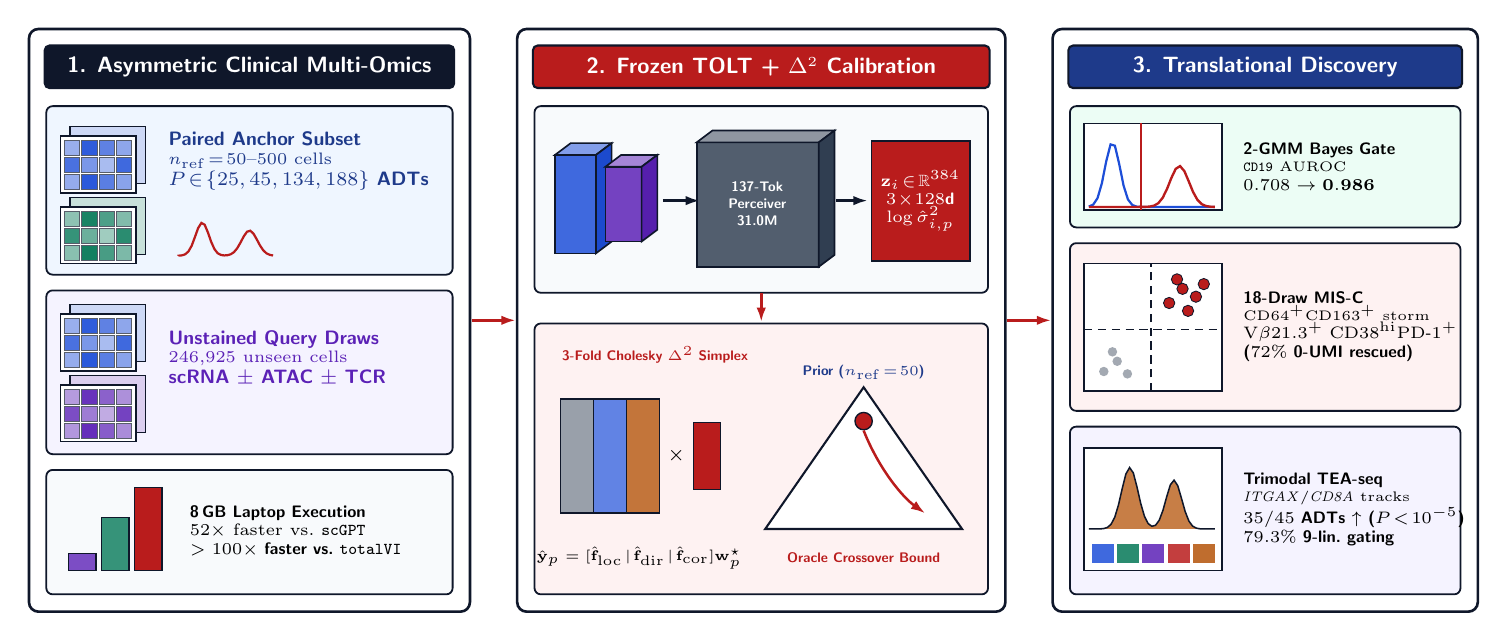
\begin{tikzpicture}[
  x=1mm, y=1mm,
  >={Latex[length=1.8mm,width=1.2mm]},
  card/.style={draw=Ink, line width=0.95pt, rounded corners=1.2mm, fill=white},
  hdr/.style={draw=Ink, line width=0.75pt, rounded corners=0.6mm, fill=Ink, text=white, font=\sffamily\bfseries\fontsize{7.8}{8.4}\selectfont, minimum height=5.4mm},
  flow/.style={->, draw=Ink, line width=0.90pt},
  flowred/.style={->, draw=Crimson, line width=0.95pt}
]

% Column 1: Asymmetric Multi-Omic Clinical Cohorts
\draw[card] (1.0,1.0) rectangle (57.0,75.0);
\node[hdr, minimum width=52.0mm] at (29.0,70.2) {1. Asymmetric Clinical Multi-Omics};

\filldraw[fill=ZoneBlue, draw=Ink, line width=0.65pt, rounded corners=0.8mm] (3.2,43.8) rectangle (54.8,65.2);
\DeckGA{5.0}{54.2}{Navy}
\DeckGA{5.0}{45.2}{Emerald}
\node[font=\sffamily\bfseries\fontsize{6.6}{7.4}\selectfont, text=DeepNavy, align=left, anchor=west] at (17.5,58.2) {Paired Anchor Subset\\[-0.2mm]\normalfont\fontsize{5.8}{6.6}\selectfont $n_{\mathrm{ref}}\!=\!50\text{--}500$ cells\\$P\!\in\!\{25,45,134,188\}$ ADTs};
\draw[Crimson, line width=0.8pt] (20.0,46.2) -- plot[domain=0:12,samples=30] (20.0+\x,{46.2+4.2*exp(-(\x-3)^2/1.5)+3.2*exp(-(\x-9)^2/2.0)});

\filldraw[fill=ZoneViol, draw=Ink, line width=0.65pt, rounded corners=0.8mm] (3.2,21.0) rectangle (54.8,41.8);
\DeckGA{5.0}{31.6}{Navy}
\DeckGA{5.0}{22.6}{Violet}
\node[font=\sffamily\bfseries\fontsize{6.6}{7.4}\selectfont, text=Violet, align=left, anchor=west] at (17.5,33.2) {Unstained Query Draws\\[-0.2mm]\normalfont\fontsize{5.8}{6.6}\selectfont $246{,}925$ unseen cells\\scRNA $\pm$ ATAC $\pm$ TCR};

\filldraw[fill=ZoneGray, draw=Ink, line width=0.65pt, rounded corners=0.8mm] (3.2,3.2) rectangle (54.8,19.0);
\filldraw[fill=Violet!80, draw=Ink, line width=0.45pt] (6.0,6.2) rectangle ++(3.5,2.2);
\filldraw[fill=Emerald!80, draw=Ink, line width=0.45pt] (10.2,6.2) rectangle ++(3.5,6.8);
\filldraw[fill=Crimson, draw=Ink, line width=0.50pt] (14.4,6.2) rectangle ++(3.5,10.6);
\node[font=\sffamily\bfseries\fontsize{6.3}{7.1}\selectfont, align=left, anchor=west] at (20.2,11.2) {8\,GB Laptop Execution\\[-0.2mm]\normalfont\fontsize{5.6}{6.4}\selectfont $52\times$ faster vs.\ \texttt{scGPT}\\$>100\times$ faster vs.\ \texttt{totalVI}};

\draw[flowred] (57.2,38.0) -- (62.8,38.0);

% Column 2: Frozen 31.0M Perceiver + Cross-Fitted Simplex
\draw[card] (63.0,1.0) rectangle (125.0,75.0);
\node[hdr, fill=Crimson, minimum width=58.0mm] at (94.0,70.2) {2. Frozen TOLT + $\Delta^2$ Calibration};

\filldraw[fill=ZoneGray, draw=Ink, line width=0.65pt, rounded corners=0.8mm] (65.2,41.5) rectangle (122.8,65.2);
\IsoSlabGA{67.8}{46.5}{5.2}{12.5}{Navy}
\IsoSlabGA{74.2}{48.0}{4.6}{9.5}{Violet}
\draw[flow] (81.5,53.2) -- (86.2,53.2);
\IsoSlabGA{85.8}{44.8}{15.5}{15.8}{Slate}
\node[font=\sffamily\bfseries\fontsize{5.5}{6.2}\selectfont, text=white, align=center] at (93.5,52.8) {137-Tok\\Perceiver\\31.0M};
\draw[flow] (103.5,53.2) -- (107.5,53.2);
\filldraw[fill=Crimson, draw=Ink, line width=0.65pt] (108.0,45.5) rectangle (120.5,60.8);
\node[font=\sffamily\bfseries\fontsize{5.9}{6.6}\selectfont, text=white, align=center] at (114.2,53.2) {$\mathbf{z}_i\!\in\!\mathbb{R}^{384}$\\$3\!\times\!128$d\\$\log\hat{\sigma}_{i,p}^2$};

\draw[flowred] (94.0,41.5) -- (94.0,37.8);

\filldraw[fill=ZoneRed, draw=Ink, line width=0.65pt, rounded corners=0.8mm] (65.2,3.2) rectangle (122.8,37.6);
% Partitioned Matrix + Simplex Triangle side by side
\filldraw[fill=Slate!50, draw=Ink, line width=0.55pt] (68.5,13.5) rectangle ++(4.2,14.5);
\filldraw[fill=Navy!70, draw=Ink, line width=0.55pt]  (72.7,13.5) rectangle ++(4.2,14.5);
\filldraw[fill=Amber!80, draw=Ink, line width=0.55pt] (76.9,13.5) rectangle ++(4.2,14.5);
\node[font=\sffamily\bfseries\fontsize{7.2}{7.2}\selectfont] at (83.2,20.8) {$\times$};
\filldraw[fill=Crimson, draw=Ink, line width=0.55pt]  (85.4,16.5) rectangle ++(3.4,8.5);
\node[font=\sffamily\bfseries\fontsize{5.4}{5.9}\selectfont, text=Crimson] at (80.5,33.6) {3-Fold Cholesky $\Delta^2$ Simplex};
\node[font=\sffamily\fontsize{5.4}{6.0}\selectfont] at (78.5,7.8) {$\hat{\mathbf{y}}_p = [\hat{\mathbf{f}}_{\mathrm{loc}}\!\mid\!\hat{\mathbf{f}}_{\mathrm{dir}}\!\mid\!\hat{\mathbf{f}}_{\mathrm{cor}}]\mathbf{w}_p^{\star}$};

\filldraw[fill=white, draw=Ink, line width=0.75pt] (94.5,11.5) -- (119.5,11.5) -- (107.0,29.5) -- cycle;
\filldraw[fill=Crimson, draw=Ink, line width=0.5pt] (107.0,25.2) circle (1.1);
\draw[->, Crimson, line width=0.90pt] (107.0,24.0) .. controls (109.0,19.0) and (112.0,15.5) .. (114.8,13.5);
\node[font=\sffamily\bfseries\fontsize{5.0}{5.4}\selectfont, text=DeepNavy] at (107.0,31.4) {Prior ($n_{\mathrm{ref}}\!=\!50$)};
\node[font=\sffamily\bfseries\fontsize{5.0}{5.4}\selectfont, text=Crimson] at (107.0,7.8) {Oracle Crossover Bound};

\draw[flowred] (125.2,38.0) -- (130.8,38.0);

% Column 3: Cohort-Wide Clinical & Trimodal Discovery
\draw[card] (131.0,1.0) rectangle (185.0,75.0);
\node[hdr, fill=DeepNavy, minimum width=50.0mm] at (158.0,70.2) {3. Translational Discovery};

% Visual 2-GMM Gate Box
\filldraw[fill=ZoneEm, draw=Ink, line width=0.65pt, rounded corners=0.8mm] (133.2,49.8) rectangle (182.8,65.2);
\filldraw[fill=white, draw=Ink, line width=0.5pt] (135.0,52.0) rectangle (152.5,63.0);
\draw[Navy, line width=0.8pt] plot[domain=0:16,samples=30] (135.6+\x,{52.4+8.2*exp(-(\x-3.0)^2/1.8)});
\draw[Crimson, line width=0.85pt] plot[domain=0:16,samples=30] (135.6+\x,{52.4+5.2*exp(-(\x-11.5)^2/3.0)});
\draw[Crimson, line width=0.8pt] (142.2,52.0) -- (142.2,63.0);
\node[font=\sffamily\bfseries\fontsize{5.9}{6.7}\selectfont, align=left, anchor=west] at (154.0,57.5) {2-GMM Bayes Gate\\[-0.2mm]\normalfont\fontsize{5.4}{6.1}\selectfont \texttt{CD19} AUROC\\$0.708 \to \mathbf{0.986}$};

% Visual MIS-C + TRBV11-2 Quadrant Box
\filldraw[fill=ZoneRed, draw=Ink, line width=0.65pt, rounded corners=0.8mm] (133.2,26.5) rectangle (182.8,47.8);
\filldraw[fill=white, draw=Ink, line width=0.5pt] (135.0,29.0) rectangle (152.5,45.2);
\draw[Ink, densely dashed, line width=0.45pt] (143.5,29.0) -- (143.5,45.2);
\draw[Ink, densely dashed, line width=0.45pt] (135.0,36.8) -- (152.5,36.8);
\foreach \x/\y in {137.5/31.5,139.2/32.8,140.5/31.2,138.6/34.0}{\fill[Slate!45] (\x,\y) circle (0.6);}
\foreach \x/\y in {145.8/40.2,147.5/42.0,149.2/41.0,146.8/43.2,150.2/42.6,148.2/39.2}{\filldraw[fill=Crimson,draw=Ink,line width=0.3pt] (\x,\y) circle (0.72);}
\node[font=\sffamily\bfseries\fontsize{5.9}{6.7}\selectfont, align=left, anchor=west] at (154.0,37.2) {18-Draw MIS-C\\[-0.2mm]\normalfont\fontsize{5.3}{6.0}\selectfont $\mathrm{CD64^+CD163^+}$ storm\\$\mathrm{V}\beta 21.3^+$ $\mathrm{CD38^{hi}PD\text{-}1^+}$\\($72\%$ 0-UMI rescued)};

% Visual TEA-seq Chromatin Track Box
\filldraw[fill=ZoneViol, draw=Ink, line width=0.65pt, rounded corners=0.8mm] (133.2,3.2) rectangle (182.8,24.5);
\filldraw[fill=white, draw=Ink, line width=0.5pt] (135.0,6.2) rectangle (152.5,21.8);
\fill[Amber!75] (135.6,11.5) -- plot[domain=0:16,samples=35] (135.6+\x,{11.5+7.8*exp(-(\x-5.2)^2/2.2)+6.2*exp(-(\x-10.8)^2/2.0)}) -- (151.6,11.5) -- cycle;
\draw[Ink, line width=0.55pt] plot[domain=0:16,samples=35] (135.6+\x,{11.5+7.8*exp(-(\x-5.2)^2/2.2)+6.2*exp(-(\x-10.8)^2/2.0)});
\foreach \xb/\cc in {136.0/Navy,139.2/Emerald,142.4/Violet,145.6/Crimson,148.8/Amber}{\fill[\cc!85] (\xb,7.2) rectangle ++(2.8,2.4);}
\node[font=\sffamily\bfseries\fontsize{5.9}{6.7}\selectfont, align=left, anchor=west] at (154.0,14.0) {Trimodal TEA-seq\\[-0.2mm]\normalfont\fontsize{5.3}{6.0}\selectfont \textit{ITGAX}/\textit{CD8A} tracks\\$35/45$ ADTs $\uparrow$ ($P\!<\!10^{-5}$)\\$79.3\%$ 9-lin.\ gating};

\end{tikzpicture}
\end{document}
